\documentclass[11pt]{article}

%  USE PACKAGES  ---------------------- 
\usepackage[margin=0.75in,vmargin=1in]{geometry}
\usepackage{amsmath,amsthm,amsfonts}
\usepackage{amssymb}
\usepackage{fancyhdr}
\usepackage{enumerate}
\usepackage{mathtools}
\usepackage{hyperref,color}
\usepackage{enumitem,amssymb}
\usepackage{graphicx}
\newcommand\tab[1][1cm]{\hspace*{#1}}
\newlist{todolist}{itemize}{4}
\setlist[todolist]{label=$\square$}
\usepackage{pifont}
\newcommand{\cmark}{\ding{51}}%
\newcommand{\xmark}{\ding{55}}%
\newcommand{\done}{\rlap{$\square$}{\raisebox{2pt}{\large\hspace{1pt}\cmark}}%
\hspace{-2.5pt}}
\newcommand{\HREF}[2]{\href{#1}{#2}}
\usepackage{textcomp}
\usepackage{listings}
\lstset{
basicstyle=\small\ttfamily,
% columns=flexible,
upquote=true,
breaklines=true,
showstringspaces=false
}
\usepackage{longtable}
\usepackage{subcaption}
\usepackage{blindtext}
\usepackage{titlesec}
%  -------------------------------------------- 

%  HEADER AND FOOTER (DO NOT EDIT) ----------------------
\newcommand{\problemnumber}{0}
\pagestyle{fancy}
\fancyhead{}
% \fancyhead[L]{\textbf{\problemnumber}}
\newcommand{\newquestion}[1]{
\clearpage % page break and flush floats
\renewcommand{\problemnumber}{#1} % set problem number for header
\phantom{}  % Put something on the page so it shows
}
\fancyfoot[L]{IE 332}
\fancyfoot[C]{Project submission}
\fancyfoot[R]{Page \thepage}
\renewcommand{\footrulewidth}{0.4pt}

%  --------------------------------------------


%  COVER SHEET (FILL IN THE TABLE AS INSTRUCTED IN THE ASSIGNMENT) ----------------------
\newcommand{\addcoversheet}{
\clearpage
\thispagestyle{empty}
\vspace*{0.5in}

\begin{center}
\Huge{{\bf IE332 Project \#2}} % <-- replace with correct assignment #

Due: April 28th, 11:59pm EST % <-- replace with correct due date and time
\end{center}

\vspace{0.3in}

\noindent We have {\bf read and understood the assignment instructions}. We certify that the submitted work does not violate any academic misconduct rules, and that it is solely our own work. By listing our names below we acknowledge that any misconduct will result in appropriate consequences. 

\vspace{0.2in}

\noindent {\em ``As a Boilermaker pursuing academic excellence, I pledge to be honest and true in all that I do.
Accountable together -- we are Purdue.''}

\vspace{0.3in}

\begin{table}[h!]
  \begin{center}
    \label{tab:table1}
    \begin{tabular}{c|ccccc|c|c}
      Student & Q1 & Q2 & Q3 & Q4 & Q5 & Overall & DIFF\\
      \hline
      Taylor Kalata & 0 & 0 & 0 & 0 & 0 & 0 & 0\\
      Alex Hart & 0 & 0 & 0 & 0 & 0 & 0 & 0\\
      Grant Laneve & 0 & 0 & 0 & 0 & 0 & 0 & 0\\
      Angelica Jovceski & 0 & 0 & 0 & 0 & 0 & 0 & 0\\
      Sam Preston & 0 & 0 & 0 & 0 & 0 & 0 & 0\\
      \hline
      St Dev & 0 & 0 & 0 & 0 & 0 & 0 & 0
    \end{tabular}
  \end{center}
\end{table}

\vspace{0.2in}

\noindent Date: \today.
}


%  -----------------------------------------

\begin{document}

\addcoversheet
\newpage
\tableofcontents


% BEGIN YOUR ASSIGNMENT HERE:
\newpage
\section{Introduction}
%Overview of the project and the required algorithms
%angelica

Machine learning enables the development of complex models to learn from data and perform various tasks such as image classification. Image classification is where a model learns to recognize and categorize images into different classes. Although, with any technology, machine learning algorithms are not immune to attacks.

Adversarial attacks have been developed to fool machine learning models by making small, changes to the input data, which cause the model to incorrectly classify the image. Adversarial attacks can be used to test the robustness of machine learning models and can also be used to deceive and manipulate models in the real world. 

In this project, we aimed to train a voting-based optimization algorithm to perform adversarial attacks on a binary image classifier. We used five different machine learning algorithms to fool the classifier, and placed them within another algorithm that assigns weights to them based on their expected performance given the image.


The ultimate goal of this project was to successfully fool the provided image classifier with a given pixel budget and to do so in less than 10 seconds per image. We evaluated our models on a set of reserved 100\% accurate data and scored them based on their successful fooled images at different budget levels. Our report will detail the rationale for selecting each of the five machine learning algorithms, how we trained them, how our optimizer allocates the votes, and why such an approach should work. We will also provide an analysis of the performance of our algorithms, their accuracy, runtime complexity, and average wall-time, as well as the lessons learned and future directions for research in this area.





\section{Purpose of Image Classifiers}
%applications of image classifiers and why they benefit different industries
%alex
In the age of Artificial Intelligence and the Internet of Things, image classifiers play an important role in providing analysis for the massive amounts of unstructured image data we obtain. Image classification is the basis for computer vision: a field in which the goal is to enable a computer to see and understand objects in photos and videos. In some cases of classification, computers access massive amounts of data and can sense details leading to a high level of accuracy in classification that can far exceed that of a human (“What is …”, 2023). 
While in this project the model is distinguishing between only grass and dandelions with a given data set, search engines such as Google are given less constraints and more data to decipher in order to predict images based on random keywords or identify objects in a reverse image search. Visual search engines are one of many applications of image classifiers. Some other prevalent examples include facial recognition, traffic control systems, and self-driving cars (Boesch, 2023).


\section{Danger of Adversary Attacks}
%explain why these attacks can be dangerous
%taylor
As mentioned above, image classifiers can be a helpful technological advance in a variety of industries. However, these classifier models can be very susceptible to adversarial attacks due to their brittle nature (PureAI Editors, 2021). Slightly changing pixels of images can completely change the model result. A simple binary image classifier to detect a dandelion will probably not be a target of an attack in the real world. But when we look at industries like medical, military, financial, security, etc, the effects of a faulty model can have serious consequences. Not only can these attacks cause incorrect classification but also doing so with reported high confidence in its prediction. For example, adversary attacks can be very dangerous with the emerging presence of self-driving cars. The "sight" of the car is made possible through deep neural networks that make up the model to classify different objects the car encounters. When the model is under attack, it can cause images to be classified incorrectly leading to accidents and injury. The self-driving car may identify a stop sign as a speed limit sign; graffiti could be identified as a person or animal in the road; another car could be mistaken for an open road. These are just some of many ways an adversary attack could potentially harm humans. It can especially be dangerous due to the fact the humans do not see any potential threat. If people are not aware of these possible attacks and their implications, it is easy to trust the models and not think twice about incorrect classifications. 
\begin{figure}[h]
\begin{center}
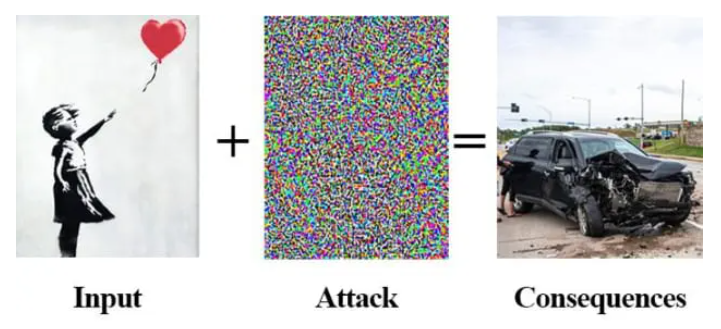
\includegraphics[width=0.75\textwidth, height=5cm]{car_accident.png}
\caption{Adversarial Attack Effect}
\label{fig:figure2}
\end{center}
\end{figure}

Because of the potential danger in many industries, defense against these attacks is being researched heavily (Wiggers, 2021). One way involves modifying a model to respond to input triggers that are used in these attacks. Researchers are implementing a Trojan horse method to test the effectiveness of their defense tactics. This allows them to better understand how the model reacts to attacks and what modifications will benefit the robustness of the neural networks. This method provides a basis for further research and techniques to boost model security. Increasing the reliability of these image classifiers will allow different fields to safely implement them to elevate the ability of machines in industry practice.

\section{Algorithm explanations}
%explain each algorithm goal/how it works
%why you picked it (fast time, accuracy, etc)
% loop invarient & runtime complexity -> IN APPENDIX, NOT THIS SECTION


% selecting each of the 5 machine learning algorithms: how you trained them, and how your optimizer allocates the votes, and why such an approach should work

% Angelica - Deep Fool
\tab The first algorithm researched was DeepFool which is a method for generating adversarial examples for deep neural networks.
The DeepFool algorithm works by iteratively perturbing an input image in the direction of the decision boundary of the model. The decision boundary is the surface that separates different classes in the feature space of the model. The algorithm calculates the minimum perturbation needed to push an input image across the decision boundary, and then moves the image in that direction. This process is repeated until the image is misclassified (Goodfellow,2015).

The DeepFool algorithm was selected because of its simplicity and effectiveness in generating adversarial examples.  Another reason DeepFool was selected is because can be used to generate targeted adversarial examples, where the attacker can specify a desired target class for the misclassification.

Specifically, the algorithm 1, was used from (Moosavi-Dezfooli,2016). 
The pseudo-code of the algorithm, consists of a loop that computes the minimum perturbation vector required to cross the decision boundary and generates a new adversarial example by moving the input image by a small amount in the direction of the perturbation vector. The loop continues until an adversarial example is found, or until the max number of iterations is reached.

%Alex - FGSM
\tab Another algorithm we researched was the Fast Gradient Sign Method or FGSM. This attack was chosen because it is a fast, single-step attack with low computational complexity (Chan, n.d.). Given the run-time constraints of this project, speed was an important factor when researching adversarial attack algorithms. The FGSM algorithm uses the sign of the gradient of the loss function with respect to the input image pixels, but in the opposite way that a typical neural network in training would. While typically the goal is to follow the direction of the gradient that minimizes loss, FGSM instead follows the direction of the gradient that maximizes loss (Ansah, 2023). In other words, FGSM nudges the pixels in the direction of the gradient that maximizes the loss to trick the classifier. In the FGSM definitive equation, a value of epsilon is multiplied by the sign of the gradient of the loss which is subtracted from original image (Chan, n.d.). The value of epsilon scales the amount of noise added to the image. The results of the scaled gradients are added to the original image generating the adversarial image. It is important to note that a higher value will result in more visually detectable defects in the image. Increasing the epsilon value will increase the likelihood of an incorrect prediction, but this project contains a pixel budget of 1 percent (Ansah, 2023). Therefore, the lowest value of epsilon able to trick the model is desirable.

%Taylor - BIM
\tab Another algorithm we researched was the Basic Iterative Method (BIM). This is an extension of the Fast Gradient Sign Method (FGSM) explained above (NueralCeption, 2023). This algorithm applies FGSM multiple times to an image with a specified step size $\alpha$, where $\alpha$ is chosen to be the intensity of one pixel. Another parameter of BIM is $\epsilon$, which limits the adversarial pertubance. This means that a maximum is set to the amount of change each selected pixel endures. The number of iterations depends on the maximum perturbance $\epsilon$ and the step size $\alpha$ to reach the maximum. This iterative approach changes the image pixels every time the FGSM algorithm is run in opposition of the orginal FGSM single large step. The attack function is passed the mean of the data, the standard deviation of the data, the model to attack, the related images, the labels from the images, epsilon, alpha, and the number of iterations. The function starts by converting the image labels to a multi-dimensional matrix of a consistent data type. We then initialize the attacked image as the original image that has been passed to the function input. The algorithm then normalizes epsilon, alpha, and the range based on mean and standard deviation of the function. The normalization converts the inputs to tensors, which are the multidimensional matrices that is the data type needed to perform operations with the images to be attacked. Once the maximum change in pixel value is calculated using $\epsilon$, the iterations of FGSM can begin over the specified number of iterations (Ansah, 2023). Each iteration of the loop with calculate the gradient with respect to the image pixels. Then it will slightly adjust the pixels toward the gradient to maximize loss between the original and attacked image. Again, this done over again for each iteration by the step size $\alpha$. Because the FGSM process is repeated many times, the BIM algorithm is going to perform slower. However, this method tends to be more successful in tricking neural network models. It also can provide more subtle changes to the images to go unnoticed by the human eye. Section 5 of our report dives further into the efficiency trade-off dilemma experienced here.


%Grant - Particle Swarm
\tab Particle Swarm Optimization, or PSO, is an optimization technique in machine learning. In PSO, particles, acting as possible solutions, swarm around a space of solutions in order to find the optimal solution (such as the minimum or maximum). The particles here mimic the behavior of swarms of animals, such as insects or birds looking for food. Essentially, the particles work together and "communicate" with each other once a discovery is found (Tam, 2021). This algorithm is less computationally intensive than some other algorithms, does not require the problem to be differentiable, and has few hyperparameters, making it more flexible (Thevenot, 2022). The algorithm starts off with the particles being located in random locations and having a random velocity in the space. This makes this algorithm a stochastic algorithm. Over time, the particles will observe their current solution, and update their velocity based on the sum of 3 factors: their current velocity multiplied by a weight factor \textit{w}, the distance between their personal best and original location all multiplied by a constant $c_{1}$ 
and random number  $r_{1}$, and a similar factor where the global best minus the original location is multiplied by random number $r_{2}$ and constant $c_{2}$. \textit{w}, $c_{1}$, and   $c_{2}$ are all user parameters that modify the behavior of the function (Tam, 2021). \textit{w} is the inertia weight constant, while $c_{1}$, and $c_{2}$ "are the cognitive and social coefficients, respectively" (Thevenot, 2022). The personal best and global best values are also updated with every iteration, and the hyperparameters can also be updated with each iteration if desired. Particle Swarm Optimization can also be applied to the context of adversarial attacks, (Mun et al., 2022). In essence, this is done by adding temporary particles using Genetic Algorithms (GA).
%Sam - Simulated Annealing 
\tab Our last algorithm is simulated annealing, a stochastic global optimization technique applicable to continuous and discrete variable problems. SA has a high attack success rate, which is why we chose it for one of our 5 attack methods.  This technique numerically approximates the global optimum in the presence of large numbers of local optima. The algorithm is basically hill-climbing, but instead of picking the best move, it picks a random move. If the selected move improves the solution, then it is accepted. If the selected move does not improve the solution, the algorithm makes the move anyway with some probability less than 1. SA is an improvement heuristic; it navigates the search space of feasible solutions by iteratively applying small perturbations to previously found solutions (Correia, 2022).  In simulated annealing adversarial attacks on image classifiers, the algorithm tries to find an input image that is similar to a given image but causes the model to misclassify it. Our implementation is an algorithm that has a perturbation operator that modifies each image by adding or subtracting noise. It also has an objective function, and the algorithm works to compare the values of the image after the perturbation operator and objective function ($delta$E). A parameter T is also used to determine this probability.  It is analogous to temperature in an annealing system.  At higher values of T, uphill moves are more likely to occur.  As T tends to zero, they become more and more unlikely, until the algorithm behaves more or less like hill-climbing.
%%%%% what we did instead %%%%%

\tab Because of the course load and time constraints of this project, we were not able to fully implement the adversary attack algorithms that are explained above. In addition to these algorithms, we researched R functions to change the appearance of images in order to fool the given model. 
%Taylor - blur and color change "algorithm"
We were able to isotropically blur the images with a certain standard deviation of the blur. As the image is blurred, the model is not always able to tell the contrast between the dandelion and surrounding grass, causing it to incorrectly classify the image. We also implemented a function to alter the image color channels. Since the grass and dandelion pictures obviously have a distinction in having the color yellow or not, changing color channels can aid in fooling the given model. By setting the green and blue channels to zero, the red channel is left. The attacked images then lack the zeroed channels, and the model has to focus on other image characteristics rather than the obvious color differences. Performance and effects can be found in the report Appendix.


%Angelica - grayscale
%%%%% ask someone to help me run it through the model



%need to ask Lucas how to interpret the results of running the test loop
%occlude function does not trick or lower accuracy as of now
%blurry function does not trick but lowers accuracy
%add noise function does not trick but lowers accuracy (have ti add isoblur to it though)
%color function drastically lowers accuracy percentage for dandelion pictures but not grass

\section{Efficiency trade-off}
%general discussion of efficiency vs quality inverse relationship
A Central Processing Unit (CPU) has a limit on how many calculations it is able to perform in a certain time frame. Therefore, the speed of every computer is limited and the runtime of each algorithm should be considered. The more operations that occur, the longer it will take for the algorithm to execute. If an algorithm is higher quality, it typically will be more complex and will therefore take more resources. However, if an algorithm is less complex, it typically will require fewer steps and take less time. In other words, an efficient algorithm may be less accurate and an accurate algorithm may be less efficient.
However, this may not be the case in all instances, such as in machine learning. In these cases, if one were to over train an algorithm on a training data set, the process of creating the model would be less efficient as training takes time and resources. In addition to that, the model would be of lower quality as it would be tailored too much on training data and would struggle to model testing data.


    
\newpage
\section{References}
\begin{verbatim}
Editors01/05/2021, P. A. I. (n.d.). Defending machine learning image classification modelsfrom attacks. Pure AI. Retrieved April 23, 2023, from 
https://pureai.com/articles/2021/01/05/defending-model-attacks.aspx#:~:text=However%2C%20it%20has%20been%20known%20for%20several%20years,the%20image%20is%20completely%20misclassified%20by%20the%20model.   

Wiggers, K. (2021, May 29). Adversarial attacks in machine learning: What they are and how to stop them. VentureBeat. Retrieved April 23, 2023, from https://venturebeat.com/security/adversarial-attacks-in-machine-learning-what-they-are-and-how-to-stop-them/ 

Boesch, G. (2023, February 24). A complete guide to Image Classification in 2023. viso.ai. Retrieved April 24, 2023, from https://viso.ai/computer-vision/image-classification/#:~:text=Image%20Classification%20is%20the%20Basis%20of%20Computer%20Vision,-The%20field%20of&text=It%20forms%20the%20basis%20for,%2C%20machine%20vision%2C%20and%20more. 

What is Computer Vision? Microsoft Azure. (2023). Retrieved April 24, 2023, from https://azure.microsoft.com/en-us/resources/cloud-computing-dictionary/what-is-computer-vision/#:~:text=Computer%20vision%20is%20a%20field,tasks%20that%20replicate%20human%20capabilities. 

Basic iterative method. NeuralCeption. (2023, April 25). Retrieved April 25, 2023, from https://www.neuralception.com/adversarialexamples-bim 

Ansah, H. (2023, April 21). Adversarial attacks on neural networks: Exploring the fast gradient sign method. neptune.ai. Retrieved April 25, 2023, from https://neptune.ai/blog/adversarial-attacks-on-neural-networks-exploring-the-fast-gradient-sign-method 

H. Mun, S. Seo, B. Son and J. Yun, "Black-Box Audio Adversarial Attack Using Particle Swarm Optimization," in IEEE Access, vol. 10, pp. 23532-23544, 2022, doi: 10.1109/ACCESS.2022.3152526.

Tam, A. (2021, October 11). A gentle introduction to particle swarm optimization. MachineLearningMastery.com. Retrieved April 25, 2023, from https://machinelearningmastery.com/a-gentle-introduction-to-particle-swarm-optimization/ 

Thevenot, A. (2022, February 17). Particle swarm optimization visually explained. Towards Data Science. Retrieved April 25, 2023, from https://towardsdatascience.com/particle-swarm-optimization-visually-explained-46289eeb2e14 

% deepfool
Goodfellow, I. J., Shlens, J., & Szegedy, C. (2015). Explaining and harnessing adversarial examples. In International Conference on Learning Representations (ICLR).

Moosavi-Dezfooli, S.-M., Fawzi, A., & Frossard, P. (2016). DeepFool: A simple and accurate method to fool deep neural networks. In Conference on Computer Vision and Pattern Recognition (CVPR) (pp. 2574-2582).

TensorFlow. (n.d.). Adversarial examples. Retrieved April 25, 2023, from https://www.tensorflow.org/tutorials/generative/adversarial_fgsm

Wong, E., Rice, L., &amp; Kolter, J. Z. (2020, January 12). Fast is better than free: Revisiting adversarial training. arXiv.org. Retrieved April 26, 2023, from https://arxiv.org/abs/2001.03994 

Pseudocode of particle swarm optimization. Research Gate. (n.d.). Retrieved April 26, 2023, from https://www.researchgate.net/figure/Pseudocode-of-Particle-Swarm-Optimization_fig1_343113703 

Morgan, A., &amp; Watson, E. (2022, May 2). A review of DeepFool: A simple and accurate method to fool Deep Neural Networks. Medium. Retrieved April 26, 2023, from https://medium.com/machine-intelligence-and-deep-learning-lab/a-review-of-deepfool-a-simple-and-accurate-method-to-fool-deep-neural-networks-b016fba9e48e 

Chan, S. (n.d.). Chapter 3 Adversarial Attack. Purdue University College of Engineering. Retrieved April 26, 2023, from https://engineering.purdue.edu/ChanGroup/ECE595/files/chapter3.pdf

Ansah, H. (2023, April 21). Adversarial attacks on neural networks: Exploring the fast gradient sign method. neptune.ai. Retrieved April 26, 2023, from https://neptune.ai/blog/adversarial-attacks-on-neural-networks-exploring-the-fast-gradient-sign-method 

Correia, A. H. C., Worrall, D. E., &amp; Bondesan, R. (2022, March 4). Neural simulated annealing. arXiv.org. Retrieved April 26, 2023, from https://arxiv.org/abs/2203.02201 

\end{verbatim}

\begin{thebibliography}{4}

\end{thebibliography}

\newpage\section{Appendix}
% Per the document: include Testing/Correctness/Verification $(1 section), Runtime Complexity and Walltime (1 section), Performance (according to the aforementioned criterion), and justification for the algorithm selected in your final implementation out of the set of implementations you tested

\subsection{Testing/Correctness/Verification}
%correctness proofs of loops from psuedocode found online (you can include the pictures)



% Angelica - Deep Fool

%cannot do correcteness // talked about loops in explanation tho

%Alex - FGSM

%Taylor - BIM
\tab For the Basic Iterative Method (BIM), the loop invariant is that the adversarial image always represents the number of pixels changed as the loop iteration that is occurring. The function begins by initializing all the variables explained in our justification section above. The adversarial image is initialized as the original image before the perturbation loop begins. For each iteration of the loop, the new gradient is calculated to determine the direction pixels will change to maximize loss. The adversarial image is then updated to reflect the changed in the pixel for that specific iteration. The for loop will terminate when the finite number of iterations is reached as the index increases by the specified step size every iteration. Once the loop terminates, the adversarial image is returned with the changes to pixels based on the number of loop iterations. 


%Grant - Particle Swarm
With Particle Swarm Optimization, the loop invariant is that SBP, or the swarm's best position will always be the most optimal position of all of the particles thus far, and p.BestPosition, or the best position of the individual particle will be the best position of the individual particle thus far. The swarm's best position will be updated to an individual particle's best position if the individual particle has a better fitness value than the current best fitness value of the swarm.


%Sam - Simulated Annealing 


\subsection{Runtime complexity/Walltime}
%explanation of how to calculate runtime
%runtime for each algorithm
%walltime is actual time it takes to run, explain difference
%sam
To calculate runtime for an algorithm, we first identify the number of operations for each iteration of the algorithm. These operations can be arithmetic operations, comparisons, and assignment operations. We represent these as weights. Next, we determine a mathematical expression in relation to the input size, n.
We then combine the weights, or number of operations, and multiply that by the mathematical expression that represents the time complexity. Walltime is a term that represents the real-time of an algorithm, in a linear sense. Start to stop, for simpler terms. Runtime, on the other hand, refers to the time it takes to execute the code or instructions, excluding the idle and/or waiting time. 

% Angelica - Deep Fool
\begin{figure}[h]
\begin{center}
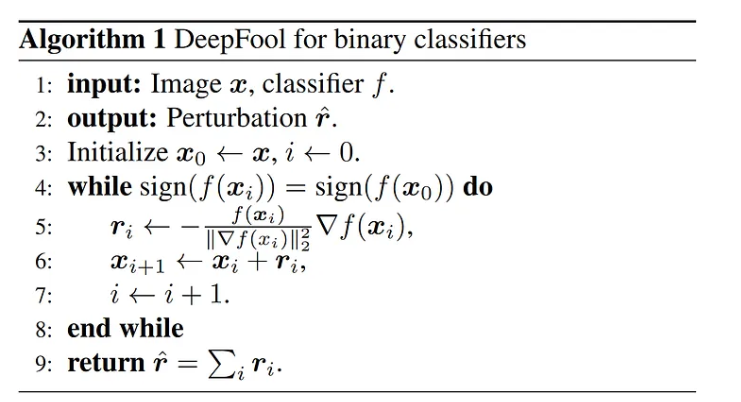
\includegraphics[width=0.55\textwidth, height=6cm]{deepfool_algorithm.png}
\caption{Deep Fool Algorithm (Morgan \& Watson, 2022)}
\label{fig:figure2}
\end{center}
\end{figure}

For DeepFool, in terms of the time complexity, a FGSM is used to solve the linear optimization problem, which has a computational complexity of O(d), where d is the dimensionality of the input data. The overall time complexity of the DeepFool algorithm can be expressed as O(Td), where T is the number of iterations required to find an adversarial example. This means that the overall runtime complexity of the DeepFool algorithm is proportional to the number of iterations required to find an adversarial example, times the dimensionality of the input data.

Although, the real runtime complexity of the algorithm will depend on factors such as, the size and complexity of the neural network being attacked, the dimensionality, complexity of the input, etc.

This is the same for Walltime. It depends on the sam factors, so it is unable to tell how long it will run for. 


%Alex - FGSM

%Taylor - BIM
\begin{figure}[h]
\begin{center}
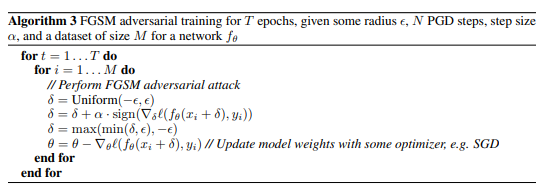
\includegraphics[width=0.75\textwidth, height=5cm]{BIM_algorithm.png}
\caption{BIM Algorithm (Wong et al., 2020)}
\label{fig:figure2}
\end{center}
\end{figure}

\tab The BIM algorithm will have a run time dependant on the FGSM run time. As seen in the figure above, BIM is composed of 2 for loops. The first loop run time will depend on the number of iterations determined from step size $\alpha$ and maximum perturbance $\epsilon$. The nested loop represents the FGSM algorithm that depends on the data set size for run time. Because of this structure, the run time complexity is in the order of $\theta$(n)=$n^2$. BIM run time will be an extension of FGSM run time by multiplying it by the number of iterations specified. 

%Grant - Particle Swarm


\begin{figure}[h]
\begin{center}
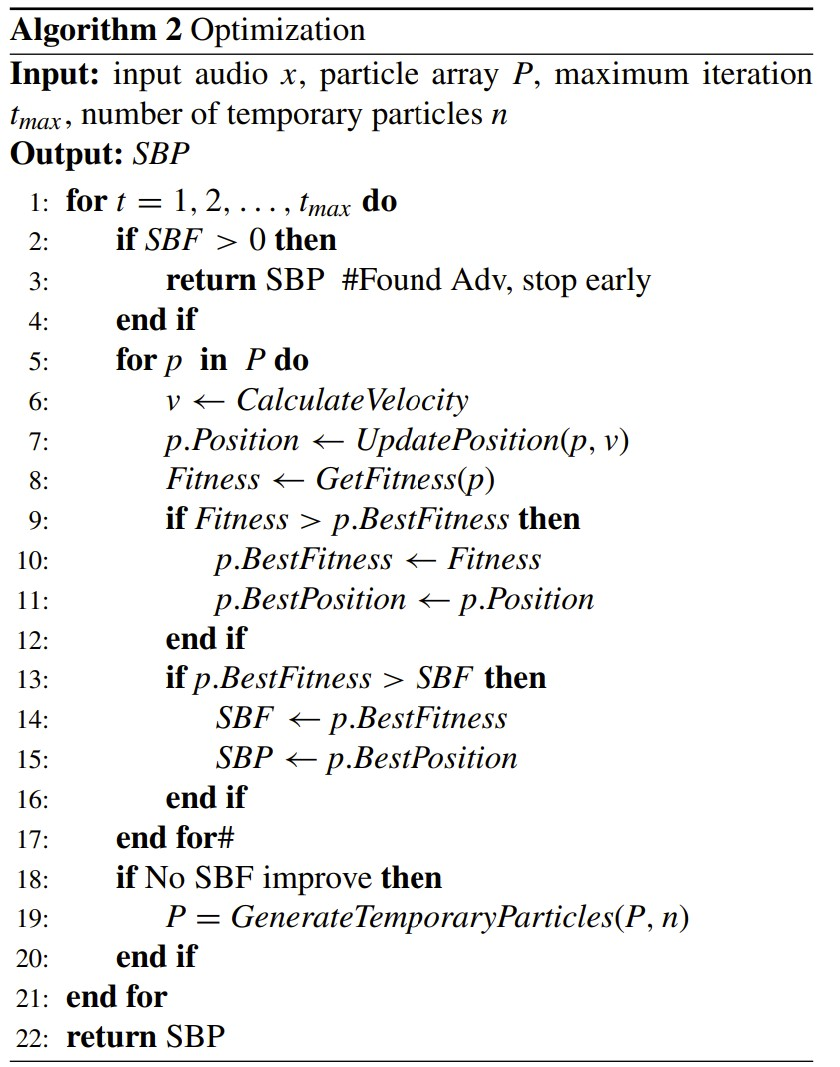
\includegraphics[width=0.5\textwidth, height=9cm]{A2.jpg}
\caption{Particle Swarm Algorithm (Mun et al., 2022)}
\label{fig:figure2}
\end{center}
\end{figure}

The run time of the algorithm highly depends on the number of specified iterations inputted by the user. Otherwise, the complexity of this algorithm seems to be in  $\theta$(n)=$nt$ time, as there is an inner and outer for loop. The first for loop is based on the maximum generation of the space in t, and the second is based on population size, n. When and if there is temporary particle generation, the algorithm will call another function running in n time, making the complexity $\theta$(n)=$ntP$ in that case, where P is the number of temporary particles.

%Sam - Simulated Annealing 

\subsection{Performance}
%before and after pictures

%Taylor - outcome of testing blurry and color

%Angelica - outcome of testing grayscale
%idek how you would go about this


\subsection{Combining Weights}

%what the weightings would be when combined into 1 algorithm


%\begin{figure}[h]
%\centering
%\subfigure[Figure 1: Label 1]{\includegraphics[width=0.4\linewidth]{picture_1.png}}
%\subfigure[Figure 2: Label 2]{\includegraphics[width=0.4\linewidth]{picture_2.png}}
%\end{figure}

\end{document}



%\https://www.sciencedirect.com/science/article/pii/S1077314298906750